\begin{proposition}
    Given the problem
    \[\text{minimize }\sum_{i=1}^{m}w_i||x^*-y_i||, x^*\in\R^n, w_1, \dots w_m \geq 0\]
    \begin{enumerate}
        \item Show that there exists a global minimum for this problem and that it can be realized by means of the mechanical model shown in figure \ref{mechanical-model}.
        \begin{figure}[h]
            \centering
            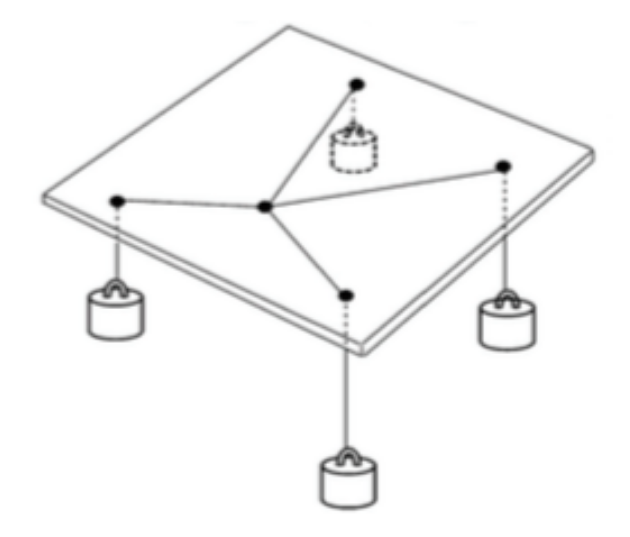
\includegraphics[width=0.5\textwidth]{../Images/mechanical_model.png}
            \caption{Mechanical model}
            \label{mechanical-model}
        \end{figure}
        \item Is the solution always unique?
        \item Show that an optimal solution minimizes the potential energy of the mechanical model defined as \(\sum_{i=1}^{m}w_ih_i\), where \(h_i\) is the height of the \(i\)th weight measured from some reference level.
    \end{enumerate}
\end{proposition}